\documentclass[]{scrartcl}

\usepackage {listings}
\usepackage[ngerman]{babel}
\usepackage[utf8]{inputenc}
\usepackage{graphicx}
\usepackage{xcolor}
\usepackage{hyperref}

\setlength{\parindent}{0em}

%opening
\title{Einkaufssimulation eines Supermarktes}
\subtitle{Fuzzy Logic - SL2 - Soft Computing - SS17}
\author{Benedikt Straube}

\begin{document}

\maketitle

\newpage

\section{Installation}
Zur lokalen Ausführung der Applikation ist eine NodeJs Installation notwendig. Diese sollte mindestens in Version 6.11.0 (\url{https://nodejs.org/}) zur Verfügung stehen.

Im nächsten Schritt sollten innerhalb des Projektverzeichnisses die notwendigen Pakete für eine lokale Ausführung installiert werden. Dies ist möglich via 
\begin{lstlisting}[backgroundcolor=\color{lightgray}]
npm install
\end{lstlisting}

Nachdem alle notwendigen Pakete installiert wurden, kann ein lokaler Server mittels
\begin{lstlisting}[backgroundcolor=\color{lightgray}]
npm start
\end{lstlisting}
gestartet werden.

Danach ist die Applikation im Browser über \url{http:localhost:4200} zu erreichen.


\section{Ausführung}
\label{ausfuehrung}
Die Applikation kann über die beschriebe Installation lokal gestartet und über den Browser bedient werden. Weiterhin wird der compilierte Code zusätzlich über GitHub-Pages gehostet. Dadurch ist die Applikation auch unter der URL \url{https://benediktst.github.io/Soft-Computing-VAWI} zu erreichen.

Vorsicht: Hier existiert zum aktuellen Zeitpunkt noch ein Bug des Routings, was bei dem Refresh der Applikation zu einer 404-Seite führt. Die Applikation kann immer wieder über die Angegebene URL erreicht werden.

\begin{figure}[htbp]
	\centering
	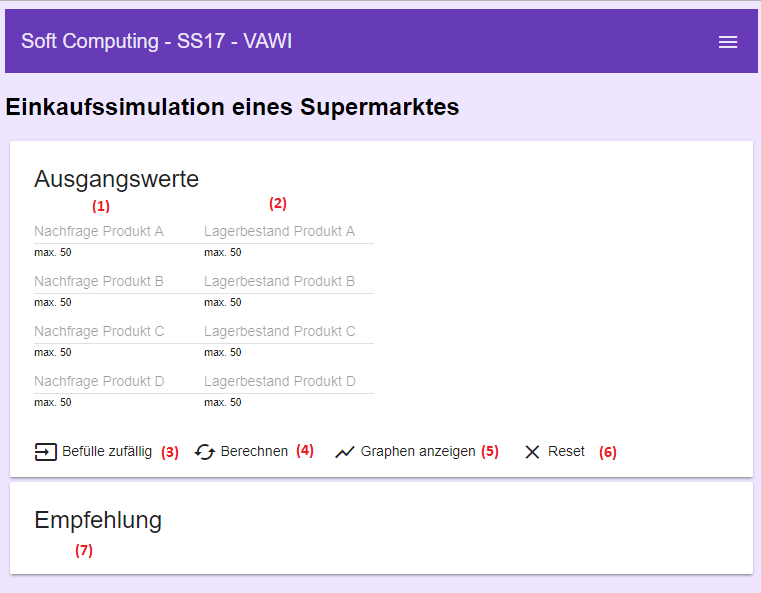
\includegraphics[width=0.7\textwidth]{res/screenshot1.png}
	\caption{Aktionsmöglichkeiten der Anwendung}
	\label{img:interface}
\end{figure}

Um die Implementierung der SL-2 zu erreichen muss innerhalb der Kopfzeile ganz rechts das Menü geöffnet und die Option SL-2 ausgewählt werden. In der Anwendung (siehe Abbildung \ref{img:interface}) können nun die Ausgangsdaten über die Eingabefelder gepflegt werden. Dabei wird im linken Block (1) die Nachfrage und im rechten Block (2) der Lagerbestand pro Produkt eingetragen. Weiterhin können durch den Button "Befülle zufällig"(3) auch zufällige Werte für alle Felder erzeugt werden. "Berechnen" (4) führt bei gefüllten Ausgangswerten eine Fuzzyfizierung durch und wendet im Anschluss alle hinterlegten Regeln auf die Datenbasis an. Zuletzt wird aus den dadurch gewonnen Werten eine Empfehlung für jedes Produkt abgegeben(7). Mittels (5) können die Graphen der Fuzzy-Sets eingeblendet werden und mittels (6) werden alle Eingaben im Formular zurückgesetzt.

\section{Aufbau der Applikation}
\label{aufbau}
Das Framework zur Implementierung ist Angular. Es nimmt keine bedeutenden Eingriffe in die Implementierung der Logik, sondern übernimmt hauptsächlich die Darstellung innerhalb des Browsers.


Die Implementierung erfolgt innerhalb nachfolgender Orderstruktur:
\begin{lstlisting}[backgroundcolor=\color{lightgray}]
src
|- app
   |- fuzzy
\end{lstlisting}
Außenstehende Komponenten sind zur Navigation und Verwaltung notwendig.

Innerhalb des Fuzzy-Ordners befinden sich folgende Dateien:
\begin{itemize}
\item fuzzy.component.css (Styling der Komponente)
\item fuzzy.component.html (Strukturierung der Komponente)
\item fuzzy.component.ts (Logik der Komponente)
\end{itemize}

Weiterhin wurde zur Trennung von Anzeige und Logik die Visualisierung der Graphen in eine Sub-Komponente fuzzy-chart.component ausgelagert. Da diese lediglich eine Komponente zur Visualisierung ist und keine eigenen Logik besitzt, wird hierauf nicht weiter eingegangen.

Im util-Ordner stehen noch weitere Klassen zur Verfügung, auf welche im Folgenden genauer eingegangen werden soll.
\begin{itemize}
	\item fuzzyController.ts (Umsetzung des Fuzzy Logic)
	\item fuzzySet.ts (Umsetzung der Fuzzyfizierten Sets)
	\item rules.ts (Hinterlegen der Regeln)
\end{itemize}

Die \textit{FuzzySet}-Klasse repräsentiert für einen Wert x die Zugehörigkeitswerte zu beliebigen Teilmengen. Die Klasse wird hauptsächlich zum Speichern und Lesen dieser Informationen verwendet. Die Methoden \textit{addPair} und \textit{getValueByKey} stehen hierfür zur Verfügung. Somit können können Teilmengen mit deren Zugehörigkeitswerten leicht  hinzugefügt und abgefragt werden.
\\

Die \textit{FuzzyController}-Klasse erhält die Fuzzy-Logic als Parameter innerhalb des Konstruktoren. In dieser sind die Bereiche der einzelnen Teilmengen mit ihren jeweiligen Zugehörigkeitsfunktionen enthalten. Die Klasse enthält die \textit{getSet}-Methode, welche zu einem Wert x die Zugehörigkeitswerte zu jeder Teilmenge in Form eines \textit{FuzzySet}-Objekts zurückgibt. Dies basiert auf der im Objekt hinterlegten Logik. Weiterhin steht die \textit{logicalAnd}-Methode zur Verfügung, welche für eine Reihe von Werten die zugehörigen Sets ermittelt und diese mit einem logischen UND miteinander verknüpft. Diese Funktion wurde zu Beginn für die Ermittlung des Gesamtlagerbestandes genutzt. Aufgrund der Ergebnisse, wurde sich dann allerdings für eine andere Methode entschieden (siehe Kapitel \ref{ergebnisse})
\\

In der \textit{Ruleset}-Klasse sind alle Regeln hinterlegt, welche auf die fuzzyfizierten Ausgangswerte angewendet werden. Jede Regel gibt dabei einen Zugehörigkeitswert zu einer der drei Ergebnismengen zur Kaufentscheidung zurück, welche gesammelt für jedes Produkt zurückgegeben werden. Die Regeln sind so aufgebaut, dass sie die für sich relevanten Zugehörigkeiten ermitteln, mit einem logischen UND verknüpfen und als Ergebnisdimension zurückgeben.

\begin{figure}[htbp]
	\centering
	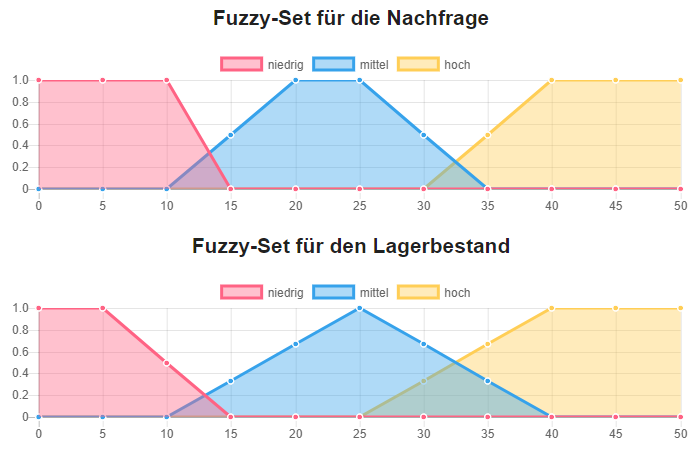
\includegraphics[width=0.65\textwidth]{res/fuzzy.png}
	\caption{Teilmengen der Fuzzy-Sets}
	\label{img:fuzzy}
\end{figure}

Die beschriebenen Klassen werden hauptsächlich durch die \textit{FuzzyComponent} verwendet. Diese ist verantwortlich für die Initialisierung und hauptsächlich zuständig für die Interaktion zwischen Frontend und Logik. Im Konstruktor werden die Eingabefelder Nachfrage und Lagerbestand für vier Produkte (A-D) erzeugt. Für de Implementierung wurde dabei eine Maximale Eingabe von 50 gewählt. Zusätzlich werden die Teilmengen der Fuzzy-Sets und deren Zugehörigkeitsfunktionen definiert. Die Zugehörigkeitsfunktionen werden dabei durch geometrische Formen wie Dreiecke oder Trapeze definiert (siehe Abbildung \ref{img:fuzzy}). Diese Funktionen sind fest im Code definiert und können nicht im Frontend angepasst werden.
\\

Die Funktionen \textit{fillrandom} und \textit{reset} werden bei den entsprechenden Buttons im Frontend ausgeführt und befüllen entweder alle Felder des Formulars mit einem zufälligen Wert oder setzten die Eingaben und das Ergebnis zurück. \textit{getTotalStockSet} ermittelt das Set für den gesamten Lagerbestand über alle Produkte, indem zuerst zu jedem Produkt einzeln die Zugehörigkeit zu den Fuzzy-Teilmengen ermittelt wird. Im Anschluss
wird für jede Teilmenge der Mittelwert über die einzelnen Produkte ermittelt.

Die \textit{calculate} Funktion übermittelt die Ausgangswerte des Frontends an das beschriebene Ruleset. Die Ergebnisse werden im Anschluss gemittelt und pro Produkt wird eine Empfehlung ausgesprochen, zu der Kaufentscheidung mit dem höchsten Zugehörigkeitswert. So steht pro Produkt eine Entscheidung der Form "Für Produkt A ist die Kaufmenge zu 74\%: Niedrig" vor.

\section{Ergebnisse}
\label{ergebnisse}
Als erstes muss angemerkt werden, dass bereits während der Entwicklung deutlich wurde, dass die Ermittlung des gesamten Lagerbestandes ein Problem darstellt. Die Information ist für die Regeln notwendig und die ersten Ansätze zur Ermittlung mit den logischen Operatoren UND und ODER führten zu ausschließlich Extremwerten. Nachdem so keine gleichmäßige Verteilung erreicht werden konnte, wurde die Berechnung auf eine Durchschnittsbildung innerhalb der einzelnen Menge angepasst. Die Ergebnisse  scheinen so besser verteilt und passen logisch trotzdem zu den Werten des Lagerbestands.
\\

Interessant ist die asymmetrische Verteilung der Teilmengen sowohl bei der Nachfrage als auch beim Lagerbestand. Dies führt dazu, dass die Empfehlungen sich nicht überwiegend im Bereich ''mittel'' zu 100\% bewegen, sondern tatsächlich eine ausreichende Varianz aufweisen. Gerade die "niedrig" Teilmengen zu beiden Sets nehmen bei einer zufälligen Verteilung zwar etwas weniger Platz ein, jedoch agieren die Regeln so, dass sowohl eine geringe Nachfrage als auch ein geringer Bestand im Lager starken Einfluss auf die Kaufentscheidung nehmen.
\\

Auffällig ist ebenfalls, dass bereits bei drei Teilmengen eine relativ hohe Anzahl an Regeln notwendig war, um sinnvolle Empfehlungen zu geben und dennoch weiteres Verbesserungspotenzial besteht. Daraus lässt sich ableiten, dass bei einer detaillierteren Unterteilung der Gesamtmenge in eine größere Zahl an Teilmengen eine stets noch höhere Anzahl an Regeln notwendig ist, um beständig sinnvolle Entscheidungen zu generieren. Gerade bei einem vollständig automatisierten System, welches in einem solchen Szenario automatisch die Bestellungen vornehmen müsste, wäre eine aufwändige manuelle Erstellung und Qualitätssicherung der Regelbasis notwendig. Es ist also definitiv bemerkbar, dass die Komplexität eines solchen Expertensystems nicht in der Umsetzung oder Konzeption der Fuzzy-Logik, sondern in der Regelbasis liegt. 

\end{document}
